\documentclass[12pt,a4paper]{article}
\usepackage[utf8]{inputenc}
\usepackage[T1]{fontenc}
\usepackage{amsmath, amssymb}
\usepackage{graphicx}
\usepackage{booktabs}
\usepackage{hyperref}
\usepackage{geometry}
\geometry{left=2.5cm,right=2.5cm,top=3cm,bottom=3cm}
\title{Calibration du modèle de Heston sur des options Bitcoin Deribit}
\date{Projet de méthodes numériques pour la finance - November 2025}
\author{Tarik Aziki, Nina Boulton, Salma Himmichi}

\begin{document}

\maketitle

\section{Introduction et problématique}

Les méthodes numériques abordées dans ce cours portent sur la résolution d'équations aux dérivées partielles et la simulation de trajectoires stochastiques pour valoriser des produits dérivés.  Le cadre de Black--Scholes, qui suppose une volatilité constante, conduit à des formules fermées pour les options européennes mais ne reproduit pas la forme en « sourire » des volatilités implicites observée sur les marchés\cite{bs_limite}.  Pour remédier à cette limitation, Heston propose un modèle où la volatilité est aléatoire et suit une diffusion à réversion vers la moyenne.  L'objectif de ce projet est de mettre en œuvre ce modèle, de le calibrer sur un jeu de données d'options Bitcoin et d'analyser sa capacité à reproduire la surface de volatilité implicite.

Le Bitcoin est un actif extrêmement volatil; les volatilités implicites associées à ses options présentent un sourire marqué.  Tester le modèle de Heston sur ces données permet d'évaluer si la seule volatilité stochastique, sans composante de saut, suffit à expliquer la réalité du marché.

\section{Modèle de Heston : théorie et rappel de Black--Scholes}

\subsection{Black--Scholes et ses limites}

Dans le modèle de Black--Scholes, le sous-jacent $S_t$ suit une diffusion géométrique
\begin{equation}
  \mathrm{d}S_t = r \, S_t \, \mathrm{d}t + \sigma S_t \, \mathrm{d}W_t,
\end{equation}
où $r$ est le taux sans risque, $\sigma$ la volatilité constante et $W_t$ un mouvement brownien standard.  Sous la mesure risque--neutre, le prix d'une option européenne s'obtient par actualisation de l'espérance de son payoff.  L'hypothèse de volatilité constante implique que l'option dépend uniquement du prix final $S_T$ et mène à la formule fermée de Black--Scholes.  Toutefois, les données de marché montrent que la volatilité implicite varie en fonction du strike et de la maturité, donnant naissance au fameux « sourire » de volatilité.

\subsection{Notion de sourire de volatilité}

Le « sourire » de volatilité désigne la variation systématique de la volatilité implicite en fonction du rapport strike/sous‑jacent (moneyness).  Sur les marchés actions, la volatilité implicite est souvent plus élevée pour les options hors de la monnaie du côté put (skew négatif).  Sur les actifs très volatils comme le Bitcoin, on observe au contraire une volatilité implicite élevée pour les strikes lointains, ce qui traduit des attentes de mouvements importants.  Les modèles à volatilité stochastique tentent de reproduire ces courbures ; la corrélation négative $\rho$ permet par exemple de générer une pente descendante du sourire.  Toutefois, un seul facteur de variance ne suffit pas toujours à produire un sourire prononcé.

\subsection{Modèle de Heston}

Le modèle de Heston introduit une dynamique stochastique pour la variance afin de corriger ce défaut.  Sous la mesure risque--neutre, le prix $S_t$ et la variance instantanée $v_t$ satisfont
\begin{equation}
\begin{cases}
  \mathrm{d}S_t = r \, S_t \, \mathrm{d}t + \sqrt{v_t}\,S_t\,\mathrm{d}W_1(t),\\
  \mathrm{d}v_t = \kappa(\theta - v_t) \, \mathrm{d}t + \xi \sqrt{v_t} \, \mathrm{d}W_2(t),
\end{cases}
\end{equation}
où $\kappa>0$ est la vitesse de réversion de la variance vers sa valeur de long terme $\theta$, $\xi>0$ la volatilité de la volatilité, $\rho\in [-1,1]$ la corrélation entre les browniens $W_1$ et $W_2$ et $v_0$ la variance initiale.  La Table~\ref{tab:params} résume l'interprétation des paramètres.

\begin{table}[h]
  \centering
  \begin{tabular}{ll}
    \toprule
    Paramètre & Interprétation \\ \midrule
    $\kappa$ & Vitesse de retour de la variance vers sa moyenne \\
    $\theta$ & Variance de long terme (volatilité moyenne $=\sqrt{\theta}$) \\
    $\xi$ & Volatilité de la variance (amplitude des fluctuations) \\
    $\rho$ & Corrélation prix--variance \\
    $v_0$ & Variance initiale \\
    \bottomrule
  \end{tabular}
  \caption{Paramètres du modèle de Heston et interprétation.}
  \label{tab:params}
\end{table}

Cette spécification permet de générer des trajectoires de prix avec une volatilité variable, donc d'obtenir des prix d'option dépendant de l'ensemble du chemin.  Heston a montré qu'il existe une formule semi‑fermée pour une option européenne en utilisant la fonction caractéristique du log‑prix, mais cette intégrale est délicate numériquement.  Dans ce projet, nous utilisons principalement la simulation de Monte‑Carlo (schéma d'Euler--Maruyama) pour estimer le prix d'un call européen.

\section{Jeu de données}

Nous utilisons le jeu de données \textit{Deribit BTC options information} disponible sur Kaggle.  Il s'agit d'un instantané de toutes les séries d'options sur Bitcoin listées sur la plateforme Deribit.  Chaque enregistrement fournit notamment le nom de l'instrument (encodant la maturité et le strike), le strike, la maturité, le type d'option (call ou put), le prix d'exercice, le prix du sous‑jacent, la volatilité implicite bid/ask et marquée et l'open interest\cite{deribit_dataset}.  Ces données sont idéales pour construire une surface de volatilité implicite et calibrer un modèle, car les options sont européennes et les volatilités implicites sont directement fournies.

\section{Préparation des données et méthode de calibration}

\subsection{Filtrage et sélection homogène}

Le fichier d'origine contient 467 options call.  Pour obtenir un ensemble homogène, nous avons réalisé un filtrage et une sélection :
\begin{itemize}
  \item \textbf{Filtrage par maturité et moneyness :} les options trop proches de l'échéance ($T<0{,}02$ an) et celles dont la moneyness $K/S_0$ sort de l'intervalle $[0{,}8,1{,}2]$ ont été écartées.  Après filtrage, nous avons désormais 141 options.
  \item \textbf{Sélection par maturités cibles :} quatre maturités représentatives ont été retenues ($\approx$ 1, 3, 6 et 9 mois).  Pour chaque maturité, quatre options dont la moneyness est la plus proche de la monnaie ont été sélectionnées.  Les maturités moyennes des groupes sont 0,065, 0,180, 0,429 et 0,678 an.  Cette sélection fournit un jeu de 16 options destiné à la calibration.
\end{itemize}

\subsection{Simulation et pricing sous Heston}

Les options sont pricées par Monte‑Carlo : on simule $n$ trajectoires du processus $(S_t,v_t)$ en discretisant l'intervalle $[0,T]$ en $N$ pas.  La variance est reflétée à zéro pour assurer sa positivité, et les incréments browniens corrélés sont obtenus par un facteur de Cholesky.  À la maturité, le payoff d'une option call est $\max(S_T-K,0)$, actualisé par $\mathrm{e}^{-rT}$.  Un module Python, développé pour ce projet, fournit les fonctions nécessaires pour simuler les trajectoires et estimer le prix par Monte‑Carlo.

\subsection{Méthode de calibration}

La calibration consiste à trouver les paramètres $(\kappa,\theta,\xi,\rho,v_0)$ minimisant l'erreur entre les valeurs du modèle et les prix ou volatilités implicites observés.  Plusieurs stratégies ont été testées :

\begin{description}
  \item[Bornes restreintes] Les paramètres étaient contraints dans des intervalles serrés ($\kappa\in[0{,}1,10]$, $\theta\in[0{,}01,0{,}5]$, $\xi\in[0{,}05,1]$, $\rho\in[-0{,}99,-0{,}1]$, $v_0\in[0{,}01,0{,}5]$).  L'optimisation par Nelder--Mead a produit une erreur moyenne $\approx3\%$, mais plusieurs paramètres ont atteint leurs bornes ($\kappa=10$, $\theta=0{,}5$, $\xi=0{,}05$, $\rho=-0{,}1$, $v_0=0{,}5$). Cela suggère que l’espace de recherche était trop limité.
  \item[Bornes élargies] Les intervalles ont été étendus ($\kappa\le20$, $\theta\le1$, $\xi\le2$, $\rho\in[-0{,}99,-0{,}05]$).  En utilisant `least\_squares` avec multi‑démarrage, nous avons obtenu $\kappa\approx0{,}59$, $\theta=1$, $\xi=0{,}05$, $\rho=-0{,}05$ et $v_0\approx0{,}50$ avec une erreur moyenne $\approx5,9\%$.  La variance de long terme atteignait sa borne supérieure (volatilité de $100$\%), ce qui reste élevé pour un actif déjà très volatil.
  \item[Bornes intermédiaires (retenues)] Les bornes ont été choisies comme compromis ($\kappa\in[0{,}5,15]$, $\theta\in[0{,}1,0{,}8]$, $\xi\in[0{,}05,1]$, $\rho\in[-0{,}9,0]$, $v_0\in[0{,}01,1]$).  La meilleure solution donnée par `least\_squares` est $\kappa\approx1{,}62$, $\theta=0{,}8$, $\xi=1$, $\rho\approx0$ et $v_0\approx0{,}498$.  L'erreur moyenne relative est $\approx6{,}3\%$ avec des paramètres jugés réalistes.
\end{description}

Le tableau \ref{tab:calib} résume ces calibrations.

\begin{table}[h]
  \centering
  \begin{tabular}{lllll}
    \toprule
    Bornes & Paramètres & Erreur moyenne \\ \midrule
    Serrées & $\kappa=10,\theta=0{,}5,\xi=0{,}05,\rho=-0{,}1,v_0=0{,}5$ & $\approx3\%$ \\
    Élargies & $\kappa=0{,}59,\theta=1,\xi=0{,}05,\rho=-0{,}05,v_0=0{,}50$ & $\approx5{,}9\%$ & \\
    Intermédiaires & $\kappa=1{,}62,\theta=0{,}8,\xi=1,\rho\approx0,v_0=0{,}498$ & $\approx6{,}3\%$ \\
    \bottomrule
  \end{tabular}
  \caption{Synthèse des différentes calibrations.}
  \label{tab:calib}
\end{table}

La calibration retenue privilégie des paramètres crédibles pour le marché des options Bitcoin : volatilité de long terme autour de 90\%, volatilité initiale de 71\% et corrélation presque nulle, ce qui reflète l’absence d’effet de levier marqué sur cet actif.

\section{Analyse des résultats numériques}

\subsection{Qualité d'ajustement et erreurs}

Avec les paramètres intermédiaires retenus, l'erreur relative moyenne entre les prix de marché et les prix modélisés est d'environ 6,3\%, et l'erreur sur la volatilité implicite d'environ 0,03.  La figure~\ref{fig:errors} présente la distribution des erreurs de prix et de volatilité implicite, ainsi qu'un diagramme de boîtes.  La plupart des erreurs de prix se situent entre 4\% et 8\%, et les erreurs de volatilité entre 0,03 et 0,05.  Les points les plus éloignés correspondent à des maturités longues et des moneyness légèrement inférieures à 1.

\subsection{Structure par terme et smiles de volatilité}

La term structure de volatilité implicite at‑the‑money (figure~\ref{fig:termstructure}) montre que la volatilité du marché augmente d'environ 0,66 à 0,77 entre 0,08 et 0,68 an.  Le modèle reproduit correctement cette pente mais surestime légèrement le niveau.  

Les smiles par maturité (figure~\ref{fig:smiles}) confirment cette observation: pour les maturités courtes et intermédiaires, le marché présente soit une pente croissante (volatilités plus élevées pour les strikes élevés) soit un creux en U, tandis que le modèle est quasi plat ou légèrement décroissant.  En maturité longue (8,1 mois), le marché affiche une forme complexe, alors que le modèle reste lisse.

\subsection{Surface de volatilité}

La figure~\ref{fig:surface} compare la surface de volatilité implicite observée à celle du modèle.  La surface du marché présente des niveaux de volatilité allant de 0,66 à 0,77 selon le strike et la maturité, avec une dépendance marquée au strike pour certaines maturités.  La surface modélisée est plus régulière : la volatilité varie principalement avec la maturité et très peu avec la moneyness, ce qui se traduit par un « plateau » plutôt qu'un vrai sourire.

\subsection{Sensibilité aux paramètres}

La figure~\ref{fig:sensitivity} illustre la sensibilité de la volatilité implicite à chacun des paramètres du modèle.  Une corrélation plus négative $\rho$ produit un sourire décroissant (pente négative), tandis qu'une corrélation proche de zéro donne une courbe plus plate.  L'augmentation de la volatilité de volatilité $\xi$ tend à aplatir le sourire.  La vitesse de retour $\kappa$ et la variance de long terme $\theta$ modifient principalement le niveau global de la volatilité implicite.  Ces sensibilités expliquent pourquoi certains paramètres atteignent les bornes lors de la calibration : le modèle utilise toute la latitude permise pour ajuster le sourire, mais cela reste insuffisant pour reproduire une courbure prononcée.

\subsection{Dynamique simulée}

La figure~\ref{fig:paths} montre quelques trajectoires simulées du prix et de la variance sous les paramètres calibrés.  Le prix du Bitcoin oscille fortement, reflétant la volatilité élevée et la volatilité de la volatilité.  La variance suit une diffusion à réversion vers la moyenne avec des pics parfois importants.  Ces trajectoires soulignent que le modèle de Heston permet de générer des scénarios de prix réalistes pour un actif crypto, mais cette variabilité ne se traduit pas forcément par un sourire de volatilité marqué.

\subsection{Complexité algorithmique}

Chaque itération de l'optimisation nécessite de simuler des milliers de trajectoires (5 000 pendant la calibration et 10 000 pour l'évaluation finale).  Il existe un compromis entre précision et temps de calcul : augmenter le nombre de trajectoires réduit le bruit Monte‑Carlo mais allonge considérablement la durée de calibration.  L'utilisation de l'algorithme `least\_squares` améliore la convergence par rapport à Nelder--Mead, et le multi‑démarrage réduit le risque de minimum local.

\section{Conclusion et perspectives}

Ce projet a permis de mettre en œuvre et de calibrer le modèle de Heston sur des options Bitcoin extraites du jeu de données Deribit.  L'étude a montré que :
\begin{itemize}
  \item Le modèle de Heston capte correctement la structure temporelle de la volatilité implicite : les volatilités modélisées augmentent avec la maturité comme sur le marché.
  \item En revanche, il reproduit mal la courbure en strike : la volatilité implicite produite par le modèle est quasi constante en fonction de la moneyness, tandis que le marché présente souvent un sourire ou une skew prononcée.  Même en ajustant les paramètres au maximum des bornes, le sourire reste trop plat.
  \item Les paramètres calibrés (variance long terme \(\approx0,8\), variance initiale \(\approx0,5\)) correspondent à des volatilités de 70\% à 90\%, cohérentes avec l'historique du Bitcoin.  La corrélation quasi nulle suggère que les variations de prix et de variance sont peu corrélées sur ce marché.
\end{itemize}

Ces conclusions soulignent les limites d'un modèle à volatilité stochastique unique pour des actifs très volatils.  Plusieurs pistes d'amélioration peuvent être envisagées : ajouter des sauts (modèle de Bates), utiliser une volatilité locale ou des modèles à deux facteurs, calibrer sur davantage de maturités et de strikes ou sur plusieurs dates pour étudier la stabilité des paramètres.  Le modèle de Heston reste cependant un étalon de comparaison utile et un outil pédagogique pour comprendre l'impact de la volatilité stochastique sur les prix d'options.

\bibliographystyle{plain}
\begin{thebibliography}{9}
\bibitem{bs_limite}
Zheng Cao et Xinhao Lin.  \emph{Improved volatility surface modeling using mixture SABR models and Bates jump–diffusion models}.  Ils soulignent que le modèle de Black–Scholes avec volatilité constante ne parvient pas à reproduire le sourire de volatilité et motivent l'introduction de modèles à volatilité stochastique.

\bibitem{deribit_dataset}
H. Sergey Frolov.  \emph{Deribit BTC options information}.  Jeu de données Kaggle fournissant des instantanés des options Bitcoin, incluant les prix, strikes, maturités et volatilités implicites.
\end{thebibliography}



\section{Annexes : figures}

\begin{figure}[h]
  \centering
  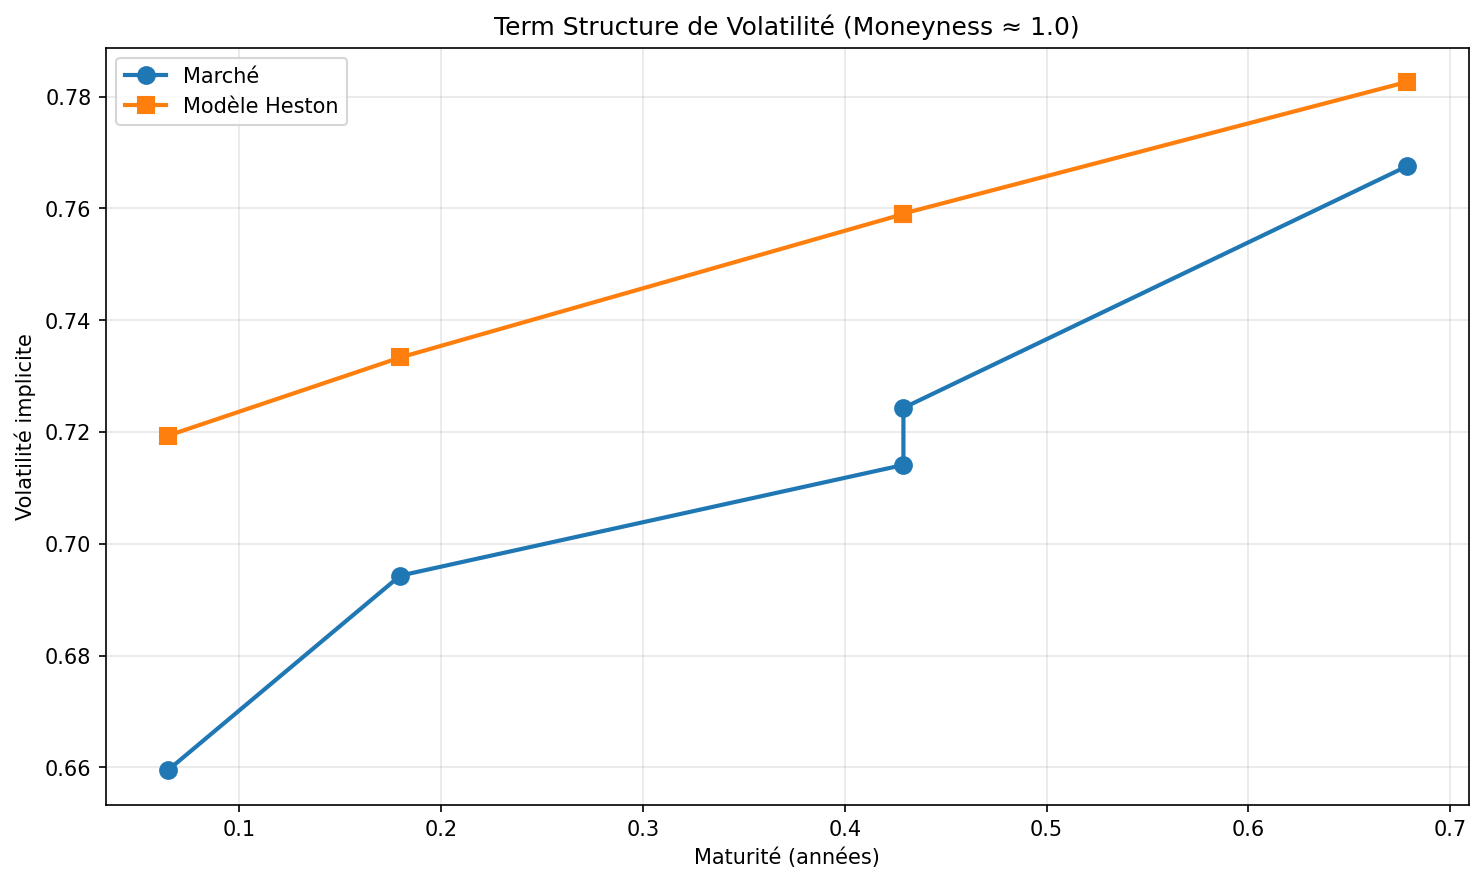
\includegraphics[width=1\textwidth]{volatility_analysis_plots/3_term_structure.png}
  \caption{Structure par terme de la volatilité implicite (marché vs modèle).}
  \label{fig:termstructure}
\end{figure}

\begin{figure}[h]
  \centering
  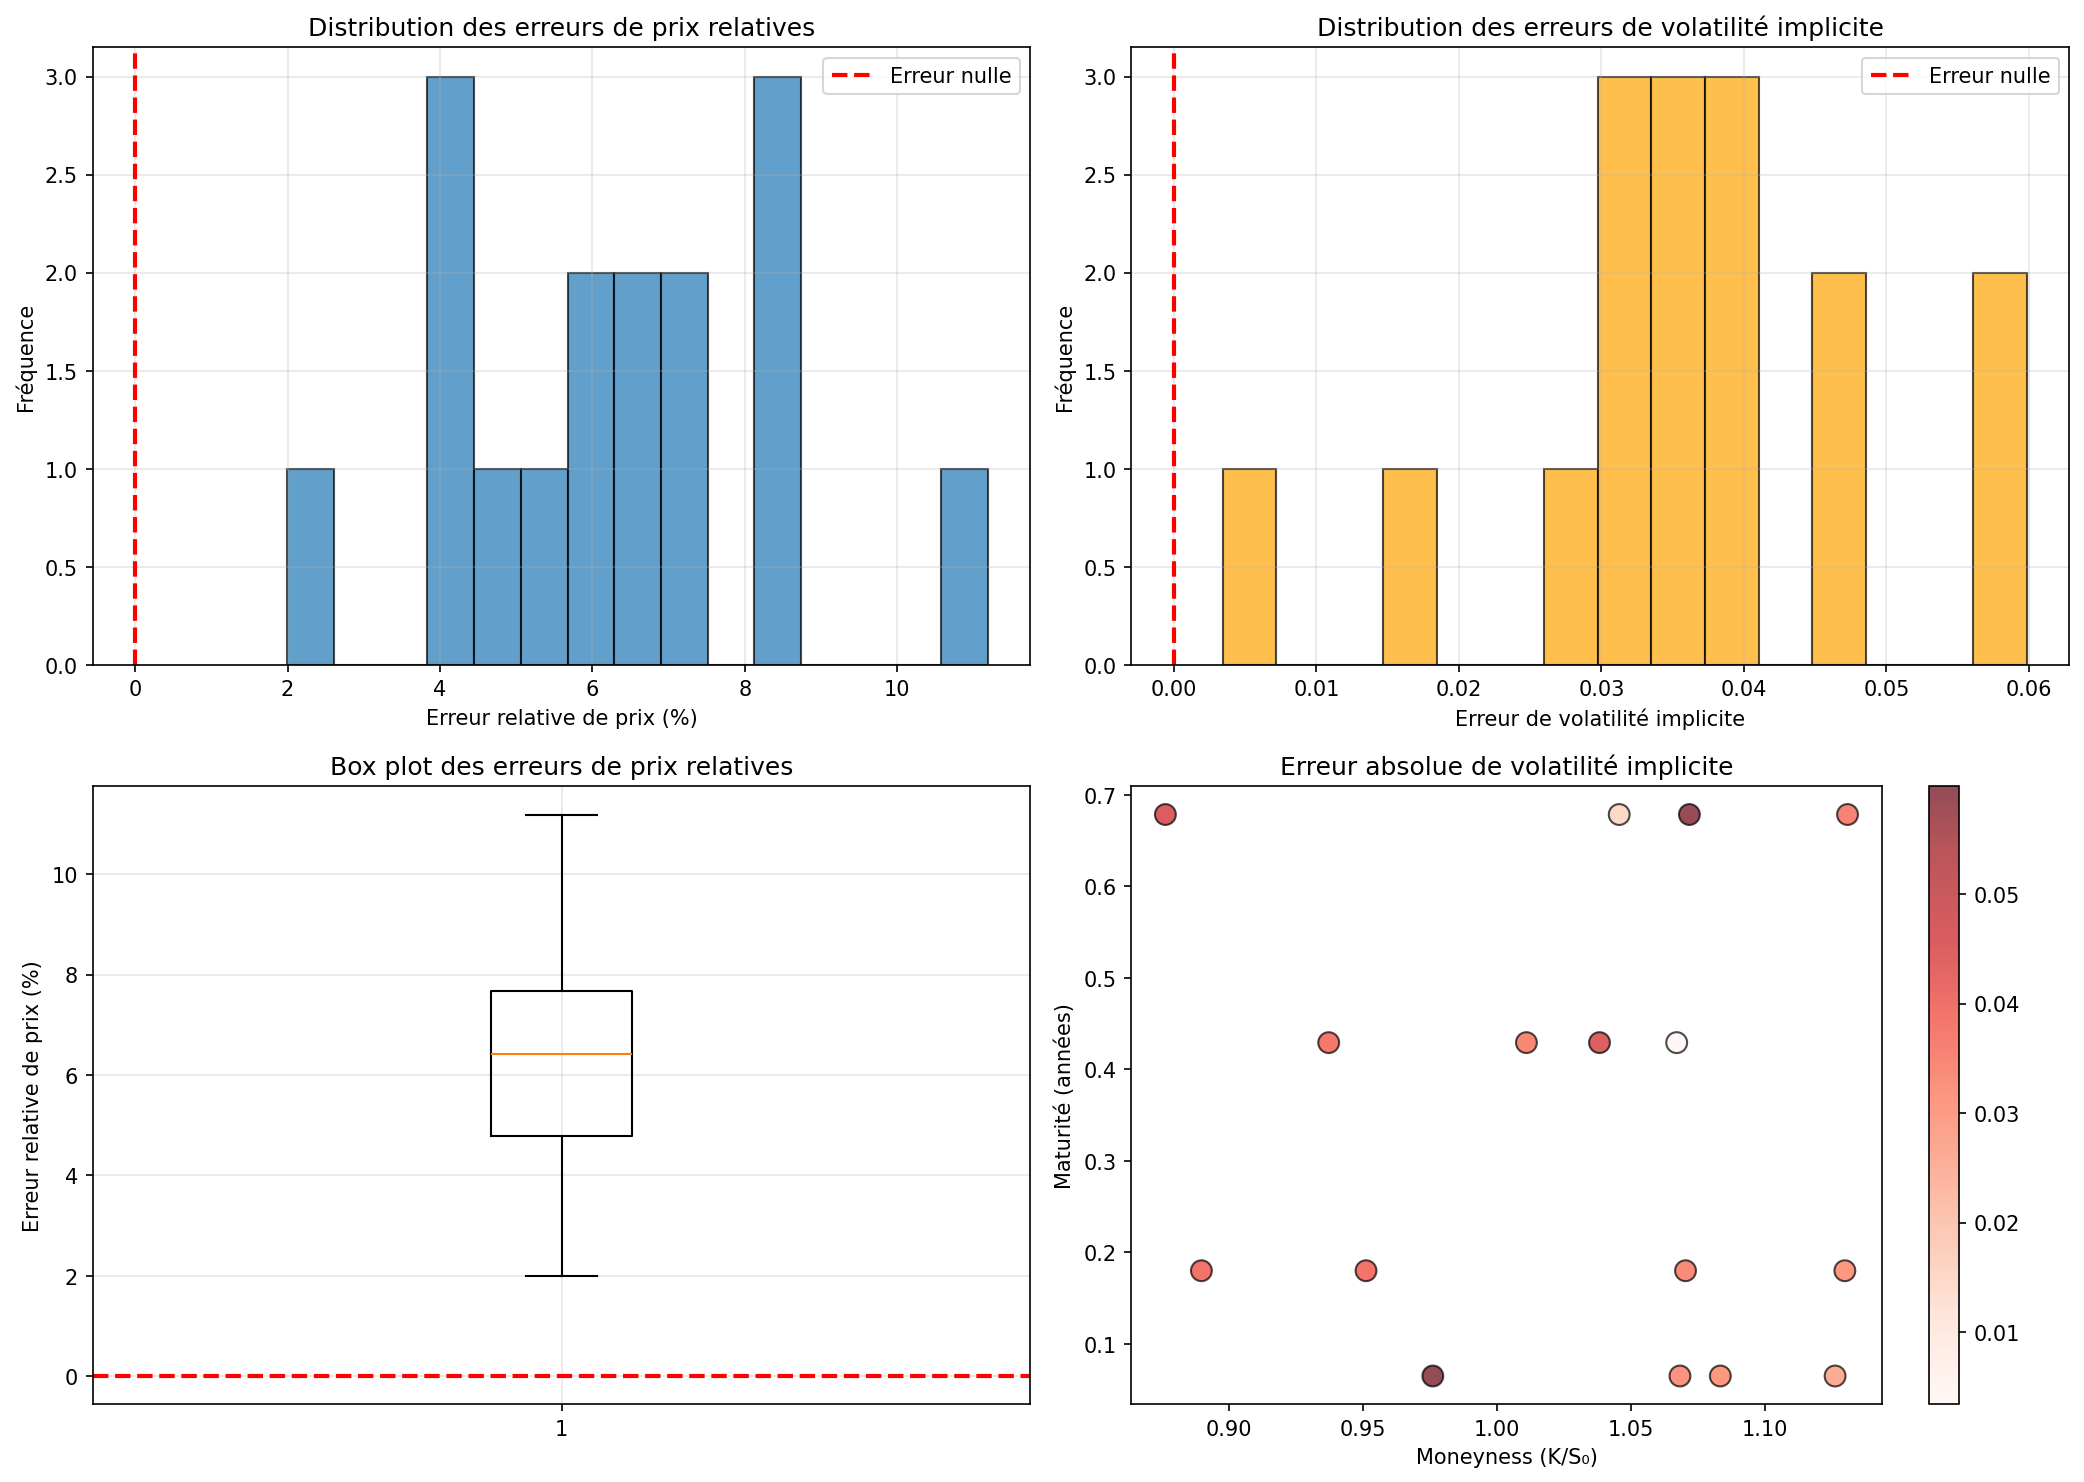
\includegraphics[width=1\textwidth]{volatility_analysis_plots/4_residual_errors.png}
  \caption{Distribution des erreurs de prix et de volatilité implicite, diagramme de boîtes et localisation des erreurs.}
  \label{fig:errors}
\end{figure}

\begin{figure}[h]
  \centering
  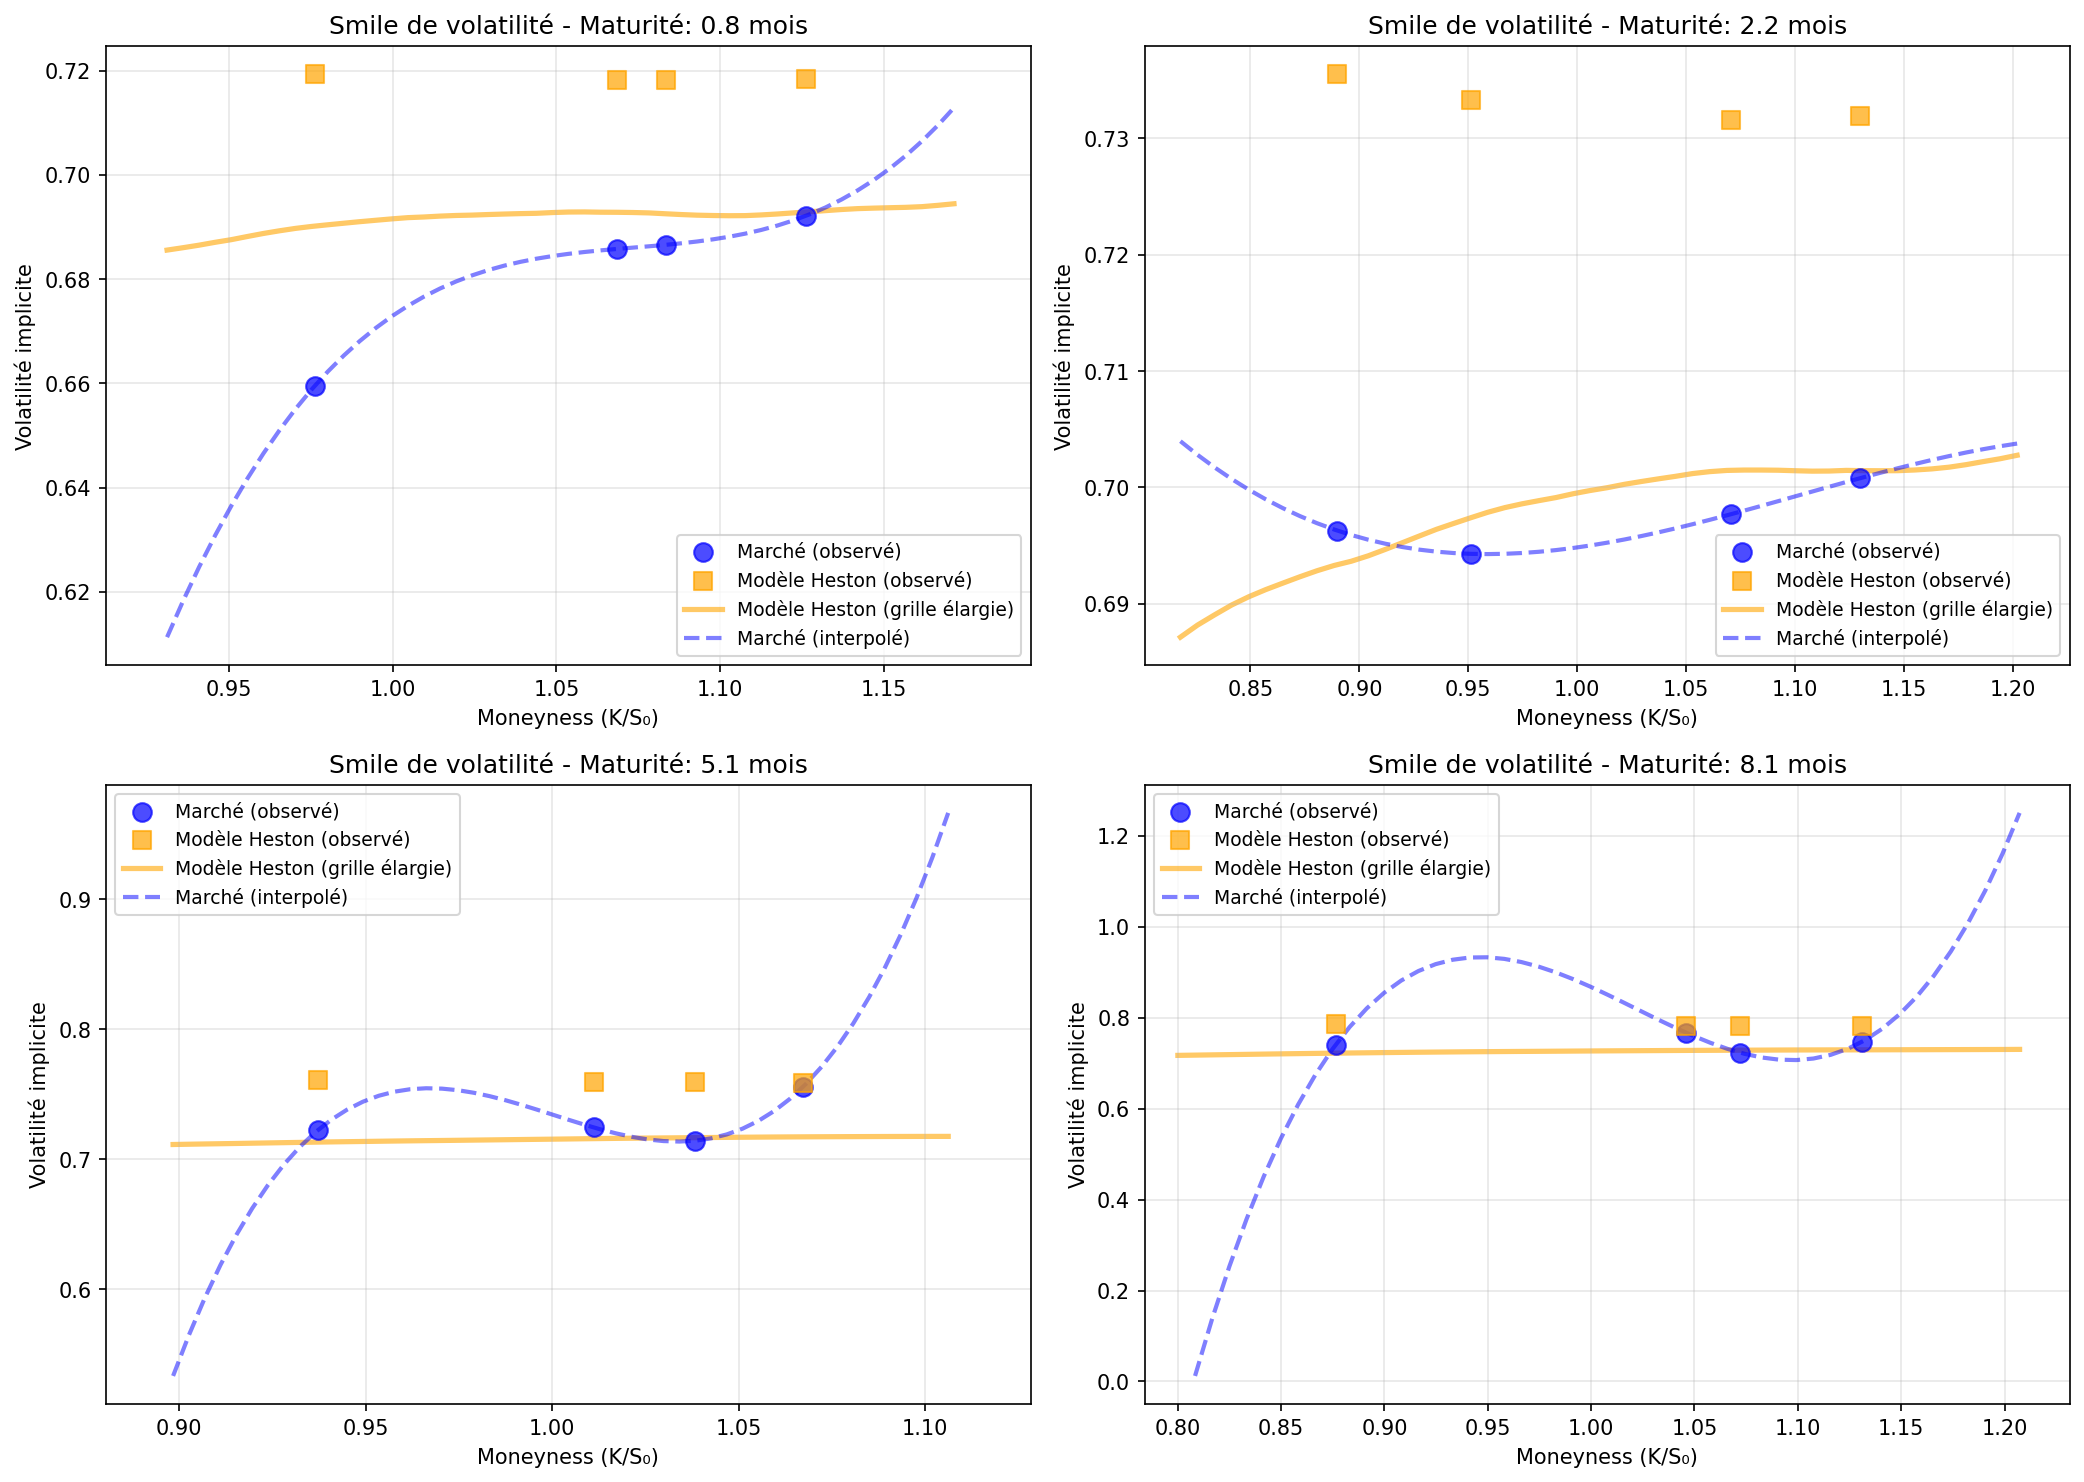
\includegraphics[width=1\textwidth]{volatility_analysis_plots/2_volatility_smiles.png}
  \caption{Smiles de volatilité pour différentes maturités : points d'observation et courbes du modèle.}
  \label{fig:smiles}
\end{figure}

\begin{figure}[h]
  \centering
  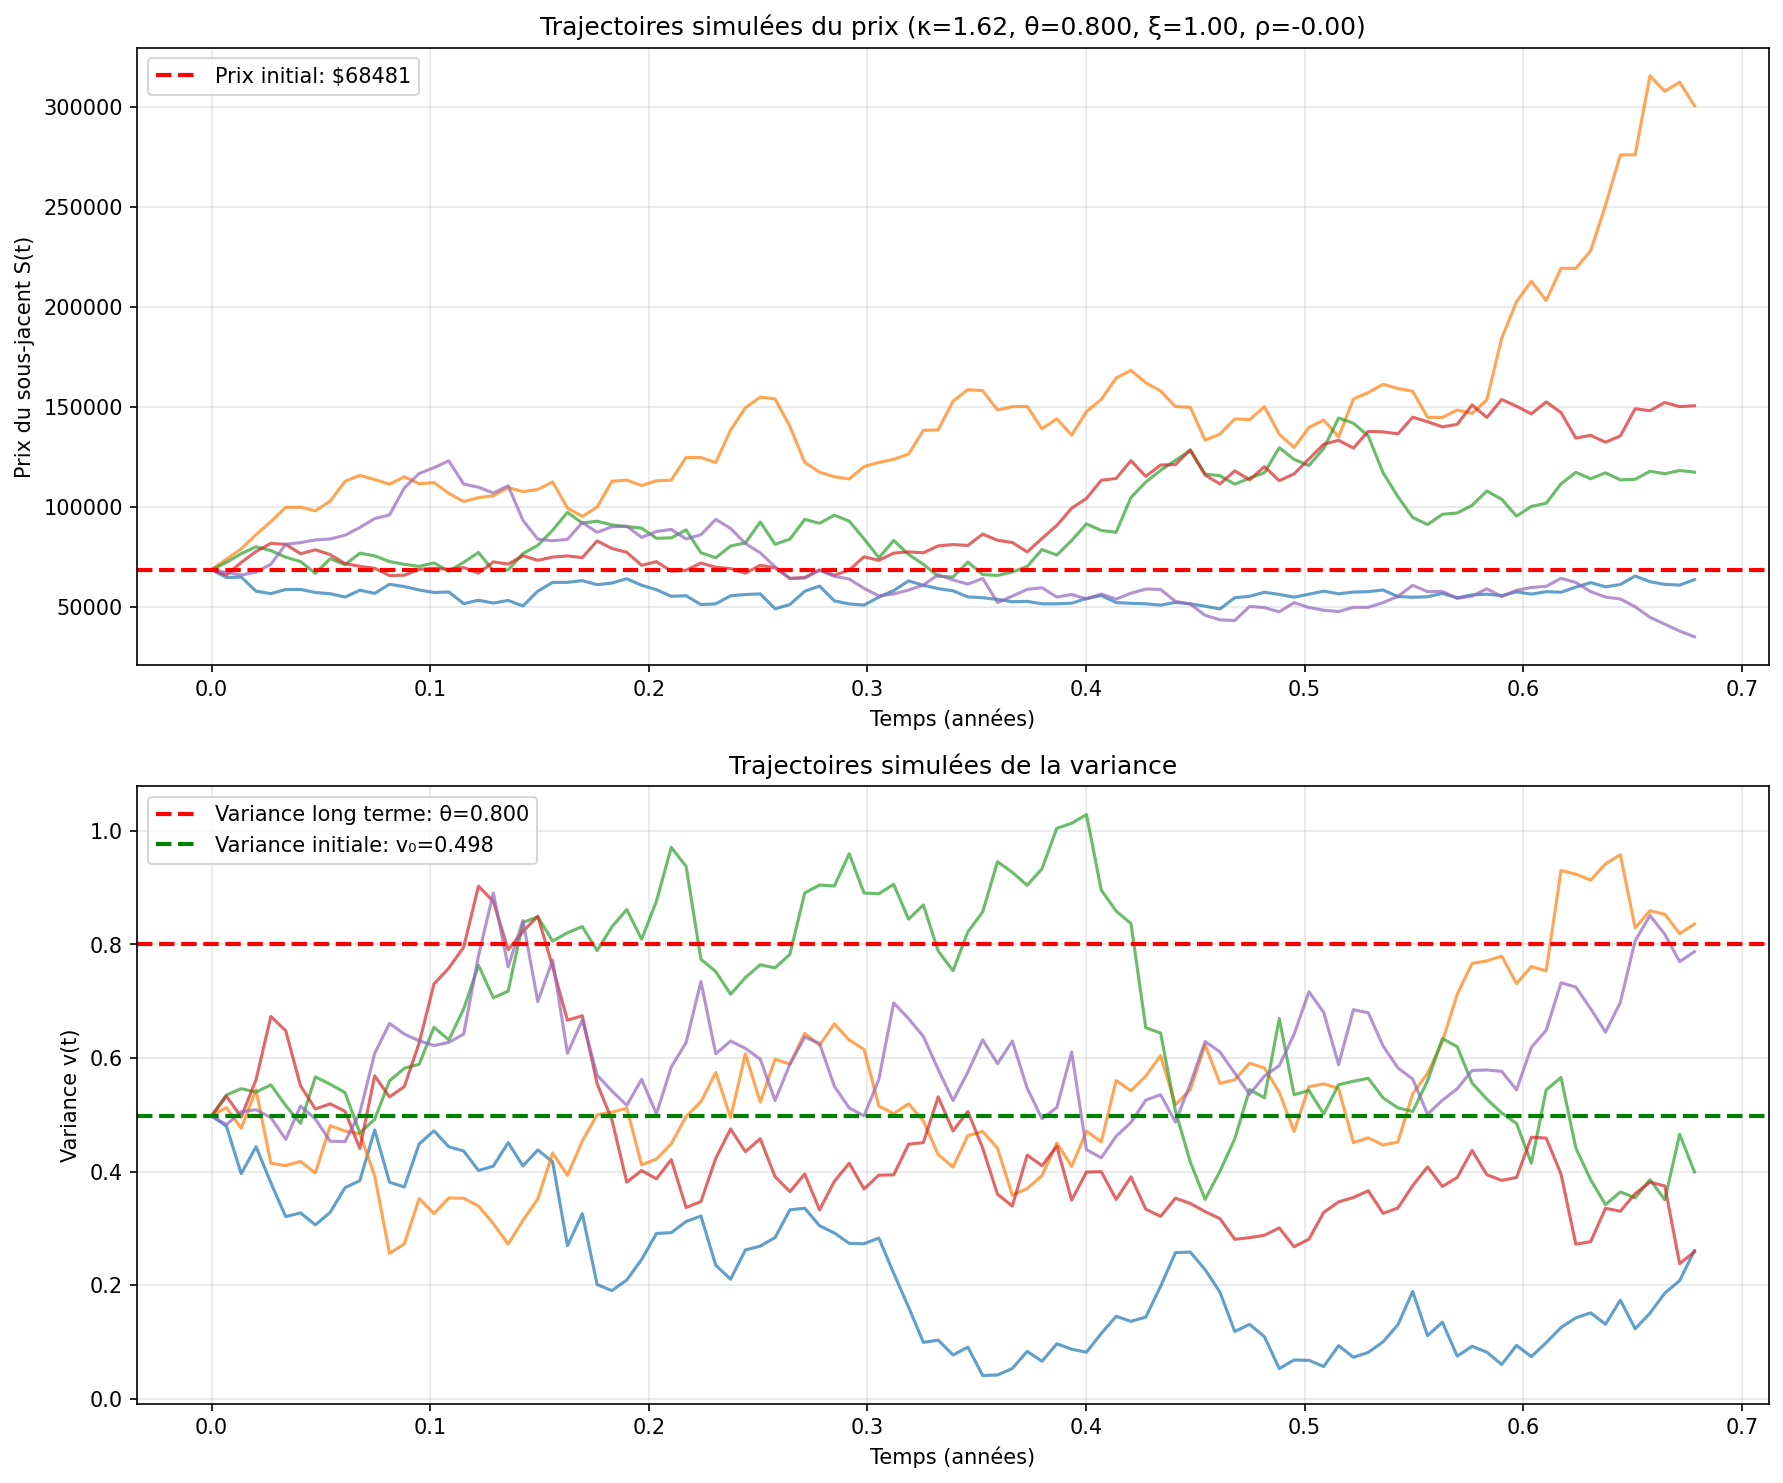
\includegraphics[width=1\textwidth]{volatility_analysis_plots/6_simulated_paths.png}
  \caption{Trajectoires simulées du prix et de la variance sous le modèle de Heston calibré.}
  \label{fig:paths}
\end{figure}

\begin{figure}[h]
  \centering
  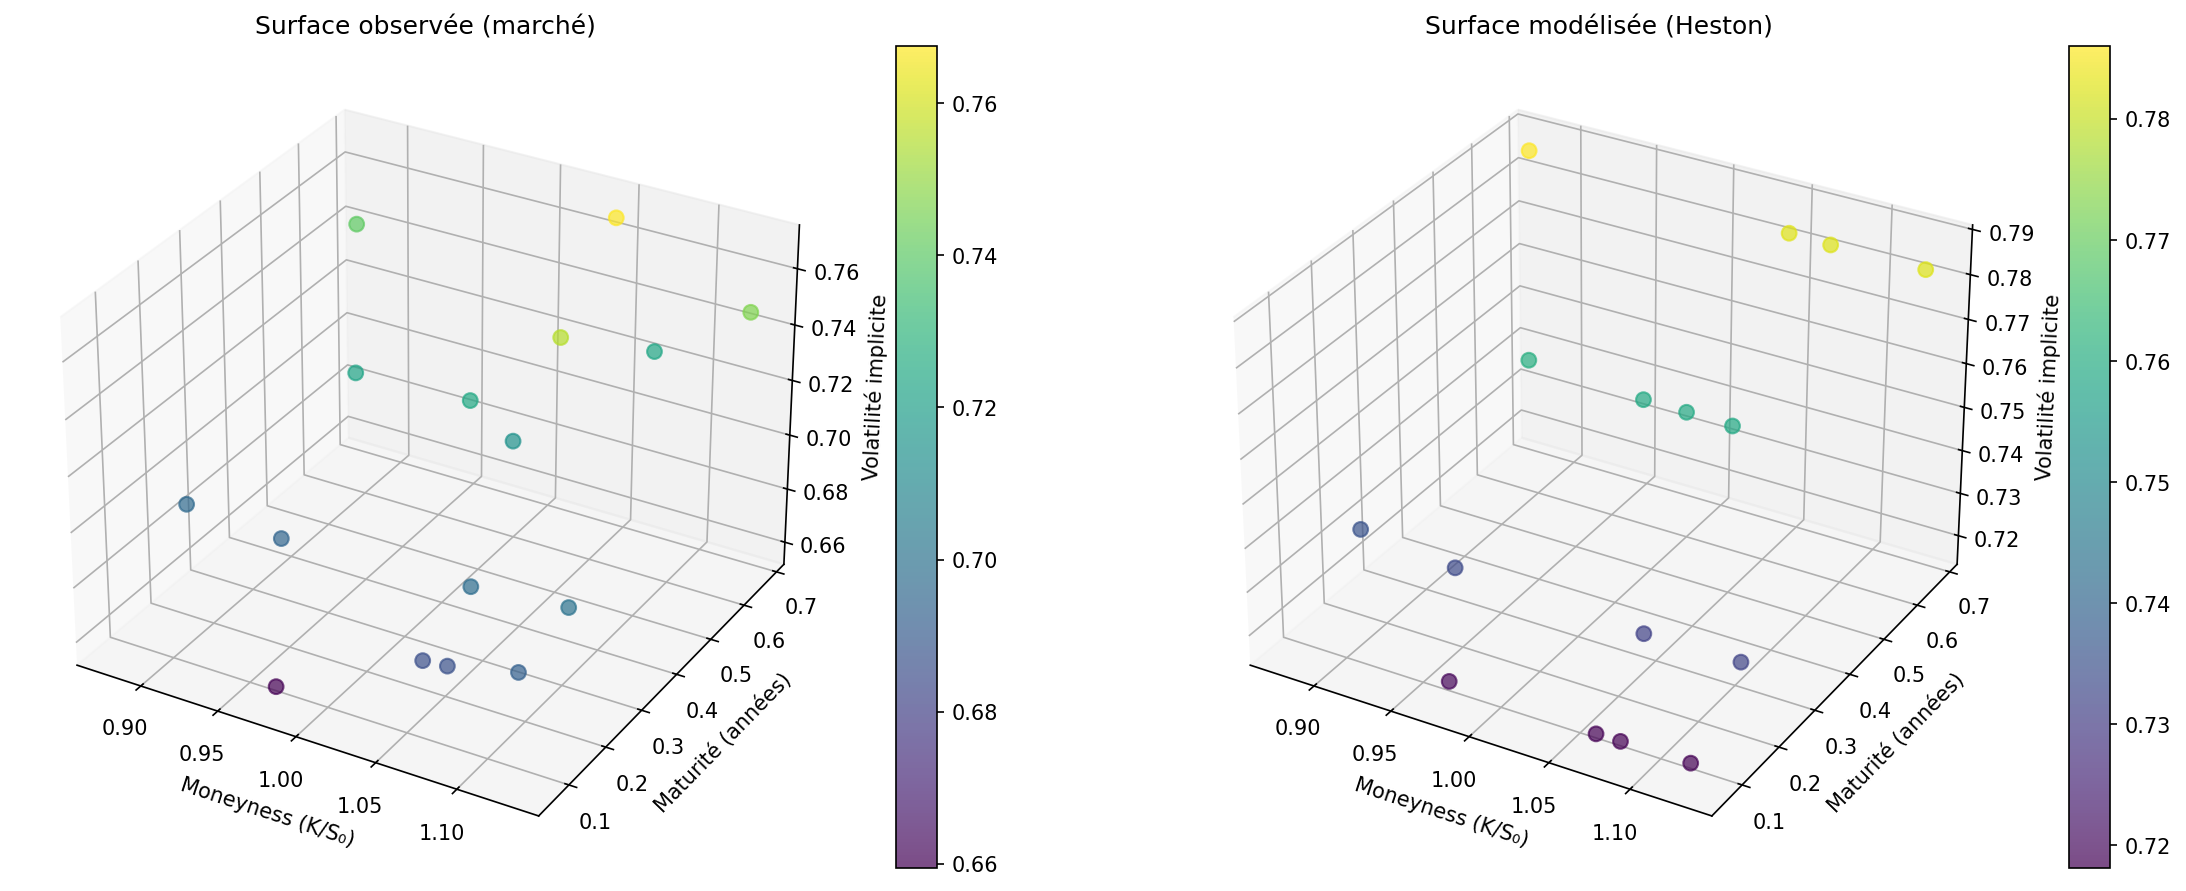
\includegraphics[width=1\textwidth]{volatility_analysis_plots/1_volatility_surface.png}
  \caption{Surface de volatilité implicite observée (gauche) et modélisée (droite).}
  \label{fig:surface}
\end{figure}

\begin{figure}[h]
  \centering
  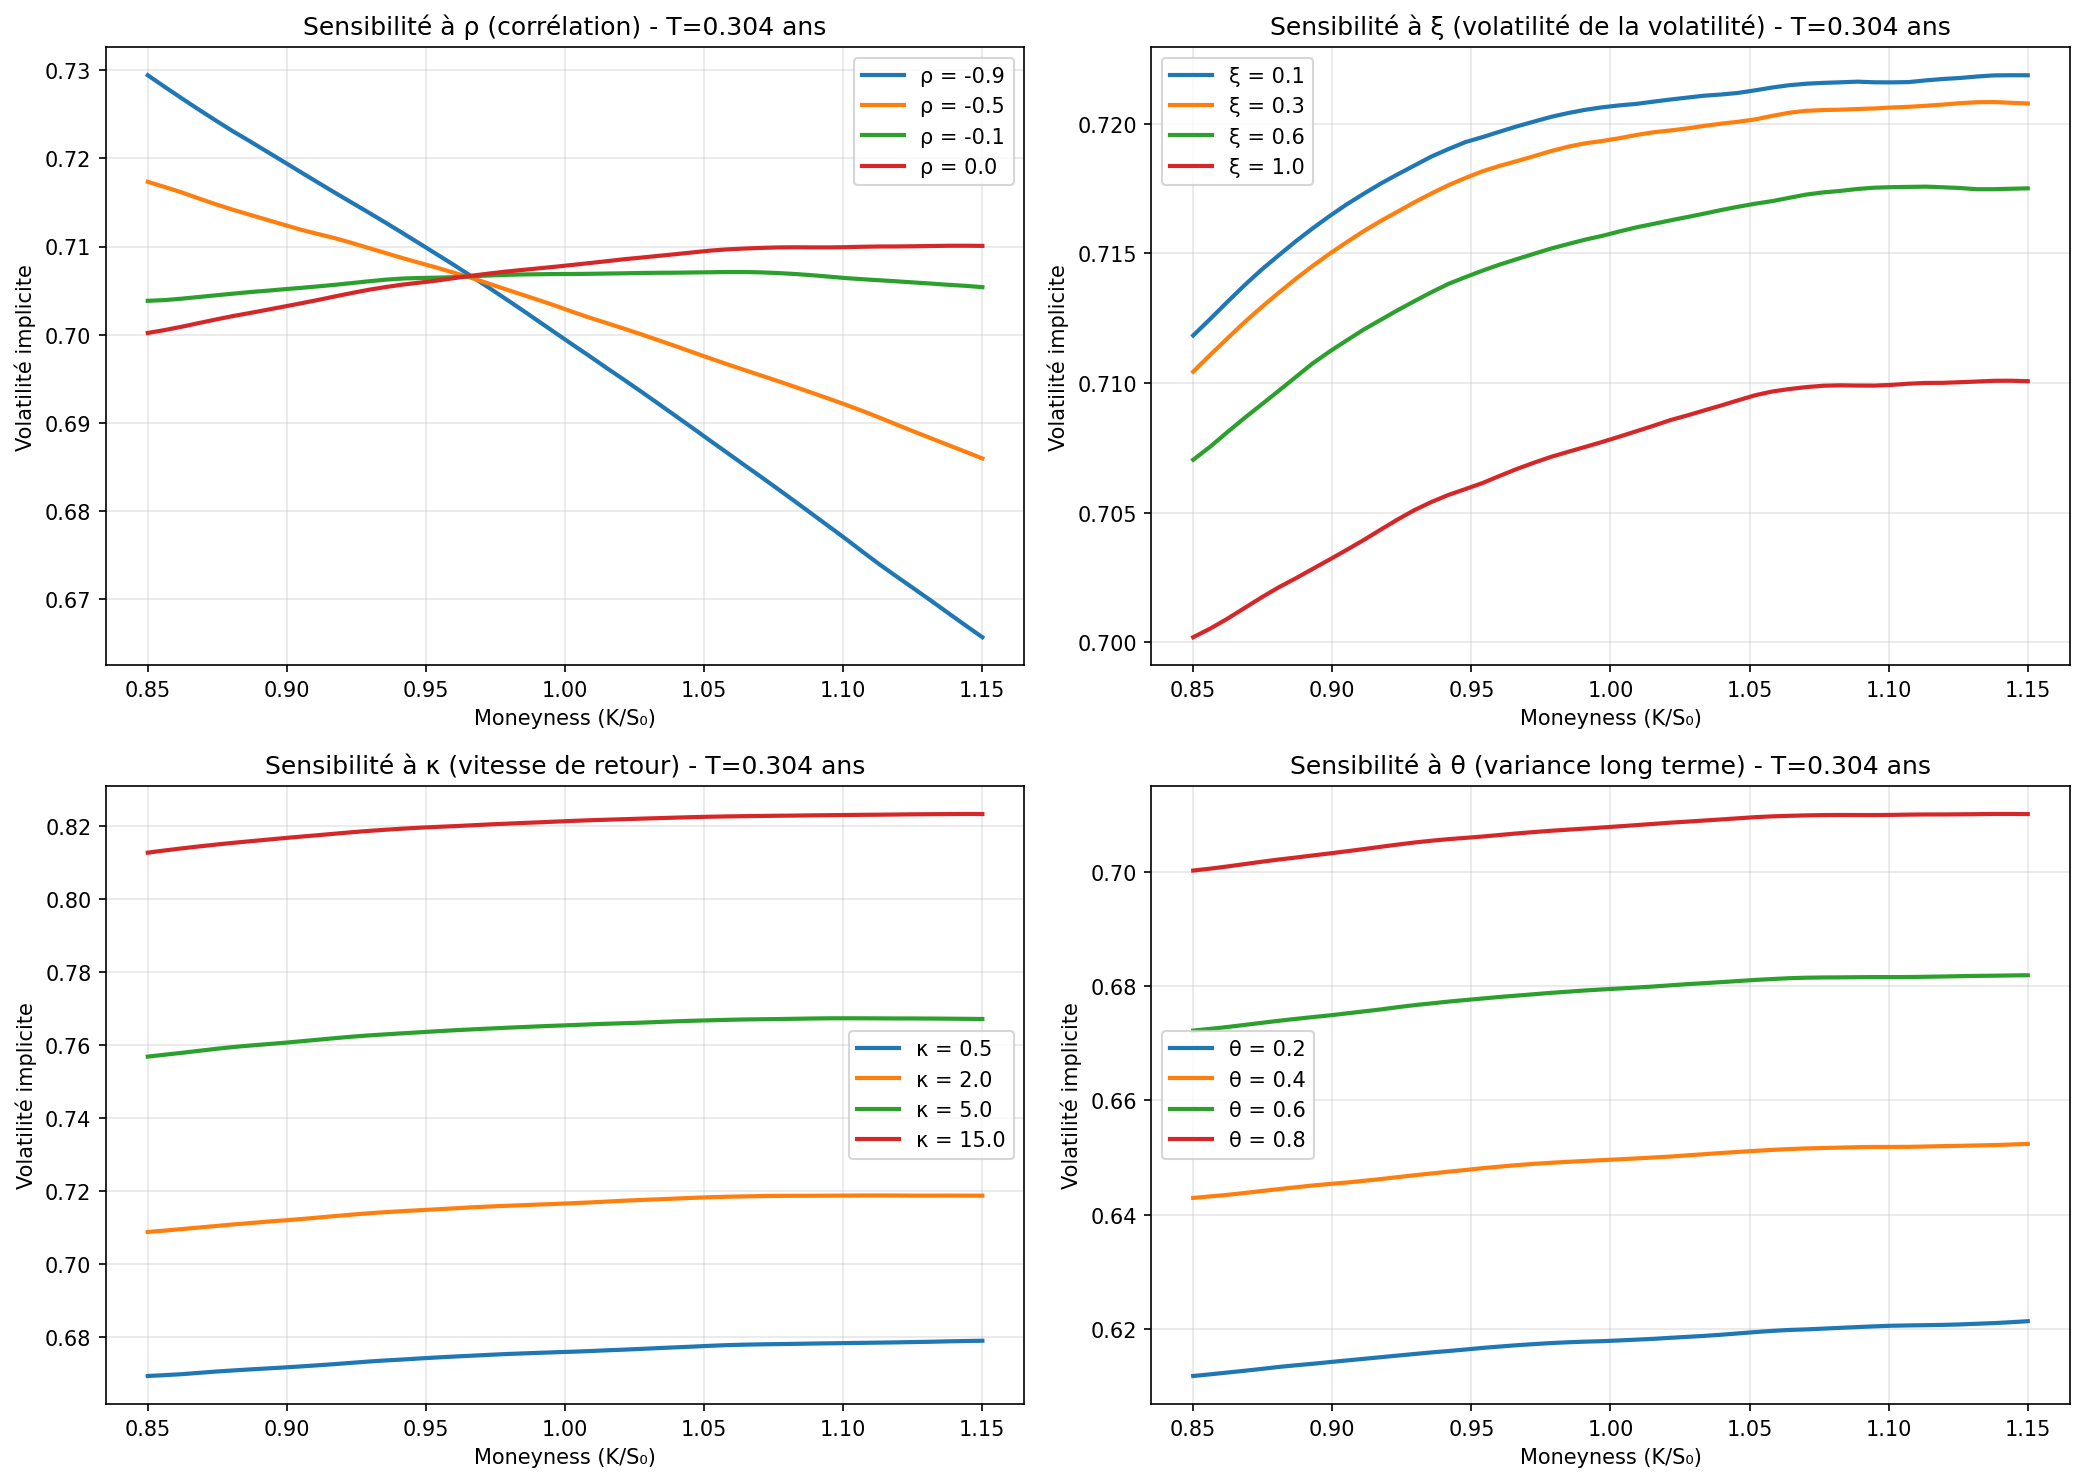
\includegraphics[width=1\textwidth]{volatility_analysis_plots/5_parameter_sensitivity.png}
  \caption{Sensibilité de la volatilité implicite aux paramètres $\rho$, $\xi$, $\kappa$ et $\theta$ pour une maturité fixe.}
  \label{fig:sensitivity}
\end{figure}




\end{document}
